\chapter{从白皮书到研究计划}
\label{chap:e28}

\begin{chapteropening}
到这里，整本书的工具箱已经装满：复振幅与相位（第 \ref{chap:e01} 章）、带宽与相干时间（第 \ref{chap:e02} 章）、泊松与散粒噪声（第 \ref{chap:e03} 章）、二阶相干 \(g^{(2)}\) 与 Siegert 关系（第 \ref{chap:e08} 章）、强度干涉与 van Cittert--Zernike 定理（第 \ref{chap:e10} 章）、从可见度到成像（第 \ref{chap:e11} 章）、量子估计与 SPADE（第 \ref{chap:e12} 章）、事件表与时钟（第 \ref{chap:e13} 章）、相关器（第 \ref{chap:e14} 章）、误差预算与可行性（第 \ref{chap:e15} 章）、再到把恒星、致密星、黑洞、瞬变当成量子光源（第 \ref{chap:e17}--\ref{chap:e20} 章）与第一代科学案例（第 \ref{chap:e25} 章）。工具齐了，本章要回答的却是一个不那么"物理"、却决定一切能否发生的问题：\textbf{怎样把一个漂亮的想法，写成一份真的能执行、也真的可能失败的研究计划？}我们会沿着一条清晰的路径走一遍——\textbf{提出科学问题 \(\to\) 选目标与方法 \(\to\) 写误差预算、估算可达精度 \(\to\) 规划仪器与数据流程 \(\to\) 排里程碑、登记风险 \(\to\) 写成计划}——每一步都把前面某一章的公式，落成 proposal 里一个可以被审查、被复现、被打分的条目。这一章的语气会稍微转向"你"的下一步行动：读完它，你应该能把一个念头改写成工作包、验收指标和失败判据。
\end{chapteropening}

\section{从科学问题出发：先选对目标，再谈仪器}
\label{sec:e28-question}

写计划最常见的失败，不是"仪器不够好"，而是\textbf{一开始就把顺序搞反了}——先爱上一台仪器或一个时髦词（"量子""纠缠""网络"），再去找题目。正确的次序永远是：先问一个能被观测证伪的\textbf{科学问题}，再问哪个\textbf{可观测量}（observable）能回答它，最后才问需要什么仪器、什么精度、什么样的目标源。

一个可执行的科学问题，通常长这样：不是"我想研究恒星"，而是"这颗快速自转星的赤道到底比两极暗多少、扁到什么程度"；不是"我想做量子天文学"，而是"这条自然激光候选线的光子统计，是热的还是相干的"。前者含糊、无法收敛；后者立刻指向一个可观测量（\(|V|^2\) 随位置角的变化、\(g^{(2)}(0)\) 偏离 1 的量），也立刻指向一套仪器需求。

选目标时，第 \ref{chap:e25} 章那三把尺子仍然管用：\textbf{亮度}决定"有没有光子"，\textbf{角尺度}决定"这些光子能不能变成参数"，\textbf{外部先验}决定"参数能不能被唯一地翻译成物理"。但写计划时还要多加一条尺子，它在纯科学讨论里常被忽略，在 proposal 里却是生死线——\textbf{失败后是否仍有产出}。一个好计划即使主目标没检出，也应留下可复用的东西：一套定标好的事件表格式、一版公开的相关器、一张校准星表、一组时间同步的 null test。把这条写进目标选择，你就不会把全部赌注押在一次可能落空的检出上。

这一步的产物很朴素，却是整份计划的地基：一句话的科学问题 + 一个明确的可观测量 + 一份"为什么是这个目标而不是那个"的排序理由。后面所有的误差预算、仪器设计、里程碑，都是在服务这一句话。第 \ref{chap:e27} 章列的那些常见误区（把多模热光当激光、把单方向基线当成能定形状、把可见度当成能直接读相位），很多都源于\textbf{在这一步偷懒}——没把"要测什么、能证伪什么"想透，就急着上仪器。

\section{近期能落地什么：把强度干涉做成常规数据产品}
\label{sec:e28-nearterm}

先说\textbf{现在就能做}的那一档。近期（可预见的这几年）最成熟、最该优先写成 proposal 的，是把已经被 VERITAS 和 MAGIC 反复验证过的强度干涉，从"一次演示"变成"可重复的数据产品" \citep{2020NatAs...4.1164A,2024MNRAS.529.4387A}。量子网络望远镜很迷人，但它属于后面的阶段（第 \ref{chap:e24} 章），近期不该占用第一批工作包。

这个阶段的主要可观测量是：二阶相干 \(\hat g^{(2)}_{ab}(\tau)\)、平方可见度 \(|V_{ab}|^2\)、每台望远镜的目标光子率、零基线对比度、背景稀释因子，以及每条基线上的协方差。问题是：怎样判断一个近期项目\textbf{到底成不成熟}？"探测器可用""望远镜够大"这种话不能写进 proposal，因为它们不可验收。我们需要一个能打分的成熟度判据。

把项目成熟度写成一个\textbf{比值向量}，每一项都是"实际能力 \(\div\) 需求"：
\begin{equation}
  \bm{r}=
  \left(
  \frac{R_\gamma}{R_{\rm req}},\;
  \frac{\sigma_{t,{\rm req}}}{\sigma_t},\;
  \frac{\beta_0}{\beta_{\rm req}},\;
  \frac{\sigma_{{\rm sys,req}}}{\sigma_{\rm sys}},\;
  \frac{N_{\rm cal}}{N_{{\rm cal,req}}}
  \right).
  \label{eq:e28-readiness}
\end{equation}
\begin{formulaexplain}
\(\bm r\) 是项目成熟度向量。每一项都是"实际能力比需求"：光子率、计时精度、零基线对比度、系统误差地板、校准样本。只有五项\textbf{同时}都 \(\ge1\)，近期项目才算闭合。任何一项 \(<1\)，都是必须先补的短板。
\end{formulaexplain}
逐个把符号、单位和量纲交代清楚，这是把 \eqref{eq:e28-readiness} 从"漂亮的向量"变成"可核账的清单"的关键。\(R_\gamma\) 是每台望远镜的有效目标光子率，单位 \(\mathrm{s^{-1}}\)，由集光面积、量子效率、滤光带宽和目标亮度共同决定；\(R_{\rm req}\) 是达到目标精度所需的光子率。\(\sigma_t\) 是望远镜之间的相对时间同步误差，单位常取 ps 或 ns；注意这一项是\textbf{需求比能力}（\(\sigma_{t,{\rm req}}/\sigma_t\)），因为误差越小越好，所以要让"需求"在分子。\(\beta_0\) 是零基线相关对比度（无量纲），衡量仪器在"两台望远镜看同一束光"时能恢复多大的相关信号；\(\beta_{\rm req}\) 是所需对比度。\(\sigma_{\rm sys}\) 是校准后残余的系统误差地板（无量纲，和 \(|V|^2\) 同单位），同样以"需求比能力"入列。\(N_{\rm cal}\) 是可用的校准星或校准观测数，\(N_{\rm cal,req}\) 是所需数目。

这个向量的价值在于它\textbf{防止单项掩盖短板}。举个反例：假设你的光子率极高，\(R_\gamma/R_{\rm req}=5\)，看起来很富裕；但如果系统误差地板 \(\sigma_{\rm sys}=3\times10^{-5}\) 却比你想测的 \(|V|^2\) 小信号还大，那么 \(\sigma_{\rm sys,req}/\sigma_{\rm sys}<1\)，项目照样不成熟——再多的光子也压不平一个系统性的偏差。强度干涉阵列的研究反复强调这一点：基线长度、\(u,v\) 覆盖、背景控制和零基线校准必须\textbf{一起}闭合，缺一不可 \citep{2006ApJ...649..399L,2013APh....43..331D,2022MNRAS.512.1722K}。

\begin{figure}[tbp]
\centering
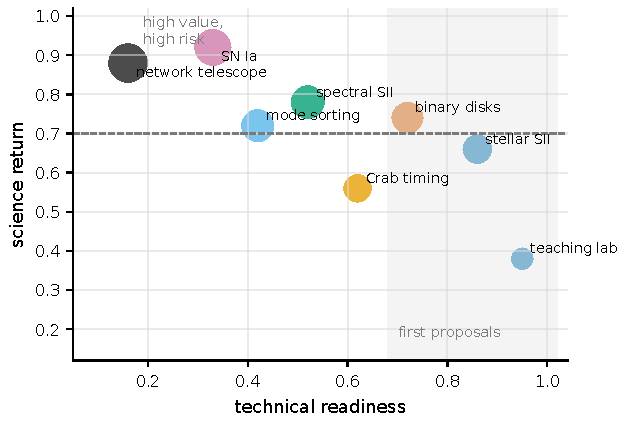
\includegraphics[width=0.86\linewidth]{figures/generated/chapter_22/ch22_roadmap_trade_space.pdf}
\caption{路线图中的技术成熟度、科学回报、成本与风险。横轴技术成熟度、纵轴科学回报，点越大表示成本压力越大。右上方且成熟度高的任务适合写成近期 proposal；左上方科学价值高但需要先做路径验证（pathfinder）的任务，属于中远期。这张图是式 \eqref{eq:e28-readiness} 那套"先看短板再谈价值"的可视化。}
\label{fig:e28-trade-space}
\end{figure}

写近期计划时，题目越具体越好。可执行的题目可以是"用四台 IACT 在 416 nm 附近测量 10--30 颗亮星的角直径，并公开相关器与校准库"，或"用同一套 pipeline 比较双星、Be 星盘和快速自转星的 \(|V|^2\) 模型"。每一篇论文都应发布：事件表格式说明、相关器版本号、time-shift null test、校准星表、基线几何、后验样本。这样即便部分目标没有检出，也留下了可复用的仪器知识——正是上一节说的"失败后仍有产出"。

\section{误差预算与可行性：先估出你能达到的精度}
\label{sec:e28-budget}

计划里最不能省、审稿人第一眼要看的，就是\textbf{误差预算}（error budget）——第 \ref{chap:e15} 章的核心工具。它回答两个问题："我这次观测最终能把可观测量测到多准？""是统计噪声、还是某个系统误差，卡住了这个精度？"没有误差预算的 proposal，等于说"我要去做，但不知道能做到多好"，几乎必被拒。

误差预算的骨架，是把各路独立误差按\textbf{平方相加}（add in quadrature）。为什么是平方相加而不是直接相加？因为若干个\textbf{互相独立}的随机误差，其总方差等于各自方差之和（这是概率论里独立随机变量方差可加的直接结果，第 \ref{chap:e03} 章讲过）。设各误差源的标准差为 \(\sigma_{\rm stat},\sigma_{\rm cal},\sigma_{\rm bg},\sigma_{\rm model},\sigma_{\rm sel}\)，则总误差为
\begin{equation}
  \sigma_{\rm tot}^2
  =
  \sigma_{\rm stat}^2
  +\sigma_{\rm cal}^2
  +\sigma_{\rm bg}^2
  +\sigma_{\rm model}^2
  +\sigma_{\rm sel}^2 .
  \label{eq:e28-error-budget}
\end{equation}
\begin{formulaexplain}
各项都是某一路误差对最终可观测量贡献的标准差（与可观测量同量纲）：\(\sigma_{\rm stat}\) 统计、\(\sigma_{\rm cal}\) 校准、\(\sigma_{\rm bg}\) 背景、\(\sigma_{\rm model}\) 模型、\(\sigma_{\rm sel}\) 选择效应。独立误差按方差相加，所以\textbf{最大的那一项主导总误差}——先去压它。
\end{formulaexplain}
逐项落地，也顺带说清各项从哪儿来。\(\sigma_{\rm stat}\) 是统计噪声，来自泊松或相关计数的有限样本，随积分时间按 \(T^{-1/2}\) 下降。\(\sigma_{\rm cal}\) 是校准误差，来自零基线对比度、时间同步、偏振与光谱响应的不完美。\(\sigma_{\rm bg}\) 是背景，来自夜天光、连续谱或伴星混入。\(\sigma_{\rm model}\) 是模型误差，来自你用来拟合的恒星盘、超新星光球、BLR 或 maser 几何本身不够真实。\(\sigma_{\rm sel}\) 是选择效应，来自触发、天气、目标挑选带来的偏差。式 \eqref{eq:e28-error-budget} 的实用读法是：\textbf{平方相加意味着最大项一票否决}——若某一项比其余大三倍，其余项开方后几乎不改变总和，你的全部精力都该去砍那一项。像 MCMC、nested sampling 或后验预测检查这些统计工具，能帮你把 \(\sigma_{\rm stat}\) 和参数后验算准，但它们\textbf{无法替代}\(\sigma_{\rm cal}\)、\(\sigma_{\rm model}\) 这些物理误差项本身 \citep{2013PASP..125..306F,2009MNRAS.398.1601F,1979ApJ...228..939C,2013ApJ...764..167S}。

误差预算里最该先估的，往往是统计项 \(\sigma_{\rm stat}\)，因为它直接告诉你"这个目标到底做不做得动"。第 \ref{chap:e15} 章给出的强度干涉信噪比是一个可以点名的已知结果（Hanbury Brown 的经典表达）：
\begin{equation}
  \left(\frac{S}{N}\right)
  =
  A\,\alpha\,n\,|V|^2
  \sqrt{\frac{\Delta f\,T}{2}} .
  \label{eq:e28-snr}
\end{equation}
\begin{formulaexplain}
强度干涉的信噪比：\(A\) 集光面积，\(\alpha\) 量子效率，\(n\) 单位面积、单位带宽的光谱光子流（谱通量密度），\(|V|^2\) 平方可见度信号，\(\Delta f\) 电子带宽，\(T\) 积分时间。关键在于信噪比只随 \(\sqrt{T}\) 增长——想把精度翻倍，积分时间要变四倍。
\end{formulaexplain}
把符号的单位摆出来：\(A\) 单位 \(\mathrm{cm^2}\)，\(\alpha\) 无量纲（典型 \(0.2\text{--}0.3\)），\(n\) 单位 \(\mathrm{cm^{-2}\,Hz^{-1}\,s^{-1}}\)（也可理解为每模每秒的光子占有数 \(\bar n_\nu\) 乘上几何因子，见第 \ref{chap:e15} 章），\(\Delta f\) 单位 Hz，\(T\) 单位 s。这条式子里藏着三条写计划时必须内化的直觉：第一，信号是 \(|V|^2\) 而非 \(|V|\)——目标一旦被部分解析、\(|V|^2\) 掉下来，信噪比\textbf{按平方}损失，这就是为什么角尺度要匹配基线。第二，信噪比只随 \(\sqrt{\Delta f\,T}\) 长——把精度提高到两倍，代价是四倍的观测时间或四倍的电子带宽，这条 \(\sqrt{\cdot}\) 律直接决定你的申请时长。第三，\(n\) 与波长、带宽有关，谱复用之所以诱人，正是因为它能在多个通道并行地累加这条 SNR（下一节）。

代一组真实数字，让可行性落地。取一对 \(100\,\mathrm{m^2}\)（即 \(A=10^6\,\mathrm{cm^2}\)）的望远镜，量子效率 \(\alpha=0.25\)，电子带宽 \(\Delta f=200\,\mathrm{MHz}=2\times10^8\,\mathrm{Hz}\)，积分时间 \(T=5\,\mathrm{h}=1.8\times10^4\,\mathrm{s}\)。这里最容易估错量级的是无量纲组合 \(A\alpha n\)：把 \(A=10^6\,\mathrm{cm^2}\)、\(\alpha=0.25\) 与一颗 \(m_V\simeq6\) 的热星在窄带下约 \(n\sim4\times10^{-11}\,\mathrm{cm^{-2}\,Hz^{-1}\,s^{-1}}\) 的谱光子流代入，得到 \(A\alpha n\sim10^{-5}\)。请特别注意这个数\textbf{远小于 1}——它其实就是热光的简并参数，也就是每模每秒的光子占有数 \(\bar n_\nu\) 乘上几何因子的量级；正因为可见光热星的 \(\bar n_\nu\ll1\)，强度干涉的信号才这么微弱、这么难做（这也是为什么要靠大面积和长积分时间硬凑）。信号取一条源被部分解析、\(|V|^2\sim0.5\) 的代表性基线（真正的零基线处 \(|V|^2\to1\)，这里已离开零基线一段、源被部分解析）。则 \(\sqrt{\Delta f\,T/2}=\sqrt{2\times10^8\times1.8\times10^4/2}=\sqrt{1.8\times10^{12}}\approx1.3\times10^6\)，于是 \(S/N\sim10^{-5}\times0.5\times1.3\times10^6\approx6.7\)，也就是几倍标准差的量级——这与 LeBohec 与 Holder 对现有一代仪器"5 小时内能对 \(m_V\simeq6.7\) 的源做到几倍标准差检出"的估算一致 \citep{2006ApJ...649..399L,2013APh....43..331D}。反过来，若目标暗 1 个星等，光子流 \(n\) 掉到约 \(40\%\)，同样时间里信噪比就掉到约 \(40\%\)，要补回来得把 \(T\) 提到约 \(6\) 倍——这类数字必须写进 proposal 的可行性小节，而不是含糊地说"我们相信能做到"。

\section{仪器与数据流程：从事件表到公开归档}
\label{sec:e28-pipeline}

估完精度，接着要回答"这条精度要靠什么仪器和什么数据流程实现"。这一节把计划从"能测多准"推进到"怎么测、数据长什么样、别人怎么复现"。

近期项目的数据产品还算简单——一个蓝光滤光片上的 \(|V|^2\) 加几条基线的协方差。但一份有远见的计划，应当规划好\textbf{数据产品会怎样长大}。中期目标是把"单通道 \(|V|^2\)"扩成\textbf{多通道事件表}：光谱分辨的强度干涉能比较谱线内外的角尺度（盘比光球大，谱线区的 \(|V|^2\) 掉得更快）；偏振分辨的相关能检查磁场几何、散射与强场辐射；皮秒级事件表能把光子统计本身当成一种新的时域数据产品。谱复用（spectral multiplexing）的吸引力在于：每个光谱通道的相干时间更长，而多个通道又能并行累加式 \eqref{eq:e28-snr} 的信噪比；代价则是数据率、通道间校准和色散模型都变复杂 \citep{2021sf2a.conf..335L,2022MNRAS.512.1722K,2024MNRAS.529.4387A}。

把多通道阶段的数据产品写成一个集合，计划才算进入了工程语言：
\begin{equation}
  \bm{d}=
  \left\{
  H_{ab}^{\nu p}(\tau),\;
  \widehat{|V_{ab}^{\nu p}|^2},\;
  C_{\nu_i\nu_j}^{p_i p_j},\;
  \bm{\Sigma}
  \right\}.
  \label{eq:e28-data}
\end{equation}
\begin{formulaexplain}
\(\bm d\) 是多通道阶段的完整数据产品，不只是 \(|V|^2\)：\(H_{ab}^{\nu p}(\tau)\) 是延迟直方图，\(\widehat{|V_{ab}^{\nu p}|^2}\) 是校准后的平方可见度，\(C_{\nu_i\nu_j}^{p_i p_j}\) 是跨频/跨偏振协方差，\(\bm\Sigma\) 是把这些量绑在一起的协方差矩阵。数据\textbf{怎样存、怎样归一化、怎样发布}，决定项目是否已到工程阶段。
\end{formulaexplain}
逐项交代含义与角色。\(H_{ab}^{\nu p}(\tau)\) 是望远镜对 \(a,b\)、频率通道 \(\nu\)、偏振通道 \(p\) 上、延迟 \(\tau\) 处的符合计数直方图——它是相关器（第 \ref{chap:e14} 章）直接吐出的原始产品，\(\hat g^{(2)}\) 就是它归一化后的形状。\(\widehat{|V_{ab}^{\nu p}|^2}\) 是从直方图里定标出来的空间相干观测量（第 \ref{chap:e10} 章的 van Cittert--Zernike 桥梁把它连到源的角结构）。\(C_{\nu_i\nu_j}^{p_i p_j}\) 是不同频率或偏振通道之间的协方差，它承载了谱线内外、不同偏振之间的角尺度对比这类"真正新"的物理。\(\bm\Sigma\) 是整套数据的协方差矩阵，拟合天体参数时必须用它，而不能假装各点独立。只写一句"我们将做多通道量子观测"是远远不够的；把 \(\bm d\) 里每个量的存储格式、归一化约定和发布方式写清楚，才是工程级的计划。

\begin{figure}[tbp]
\centering
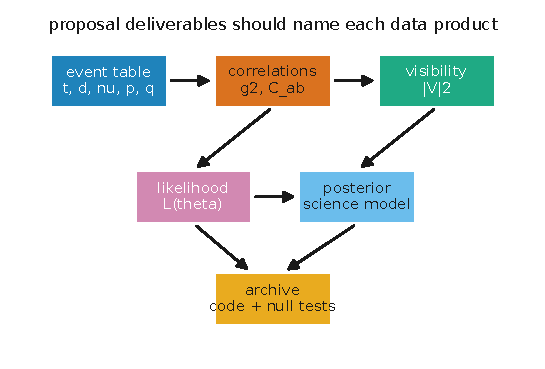
\includegraphics[width=0.88\linewidth]{figures/generated/chapter_22/ch22_data_product_stack.pdf}
\caption{从 proposal 到公开数据的产品链。事件表保留每个光子的到达时间、望远镜、频率、偏振与质量标记；相关器把它变成 \(g^{(2)}\) 与协方差；空间模型给出 \(|V|^2\)；似然与后验把它连到天体参数；归档层要包含代码、版本号与 null test。式 \eqref{eq:e28-data} 里的每个量，都对应这条链上的一环。}
\label{fig:e28-data-products}
\end{figure}

规划数据流程时，有一个贯穿全书的原则值得写进计划的第一页：\textbf{事件表是共同语言}。无论是课堂上的桌面 HBT 演示（第 \ref{chap:e26} 章）、小口径路径验证，还是大设施观测，它们都可以共用同一套"到达时间 + 望远镜 + 频率 + 偏振 + 质量标记"的事件表格式和同一版相关器 \citep{2016SPIE.9907E..0NZ,2025MNRAS.537.2527M}。这意味着你在计划里定义好的数据格式，能让教学、pathfinder 和主设施无缝衔接——这本身就是降低风险、提高可复现性的设计。

\section{风险与里程碑：让计划可以失败，但失败得有价值}
\label{sec:e28-risk}

一份计划如果只写"我们将做什么、预期看到什么"，它其实还没准备好面对现实。现实里目标会比预期暗、系统误差会卡在某个地板、瞬变会触发得太晚。成熟的计划要主动写清\textbf{里程碑}（把成功拆成可验收的节点）和\textbf{风险登记}（把可能翻车的地方连同缓解方案一起列出）。

先说里程碑。一个可执行的里程碑，必须\textbf{同时}指定"测什么"和"算成功的标准是什么"，否则它只是一句愿景。把它写成一个五元组：
\begin{equation}
  m_j=
  \left(
  O_j,\;
  \sigma_{O,j}^{\rm goal},\;
  T_j,\;
  N_{{\rm null},j},\;
  D_{{\rm release},j}
  \right).
  \label{eq:e28-milestone}
\end{equation}
\begin{formulaexplain}
\(m_j\) 是第 \(j\) 个里程碑：\(O_j\) 是要测的可观测量，\(\sigma_{O,j}^{\rm goal}\) 是要达到的目标精度，\(T_j\) 是完成日期或所需观测时间，\(N_{{\rm null},j}\) 是必须通过的 null test 数，\(D_{{\rm release},j}\) 是要发布的数据产品。一个里程碑\textbf{同时钉住}观测量、精度、时间、验证与交付，路线图才不会停在口号上。
\end{formulaexplain}
逐项落地并给出典型取值。\(O_j\) 是可观测量，例如 \(g^{(2)}(0)-1\)、\(|V|^2\)、谱线内外角尺度比、或距离 \(D_A\)。\(\sigma_{O,j}^{\rm goal}\) 是目标精度，直接来自上一节的误差预算 \eqref{eq:e28-error-budget}——里程碑的精度目标不能拍脑袋，必须是误差预算算得出的数。\(T_j\) 是完成日期或所需机时。\(N_{{\rm null},j}\) 是 null test 数：近期项目可要求 \(N_{\rm null}\ge2\)（time-shift 和 off-source 两种）；中期多通道项目应升到 \(N_{\rm null}\ge4\)（再加 off-band、错偏振、注入-恢复）；远期网络项目还要包含链路保真度和存储退相干的独立验收。\(D_{{\rm release},j}\) 是交付的数据产品，例如式 \eqref{eq:e28-data} 里的某个子集加上代码与版本号。把这五项写全，评审就能逐条判断你哪个节点算过关、哪个还欠账。

\begin{figure}[tbp]
\centering
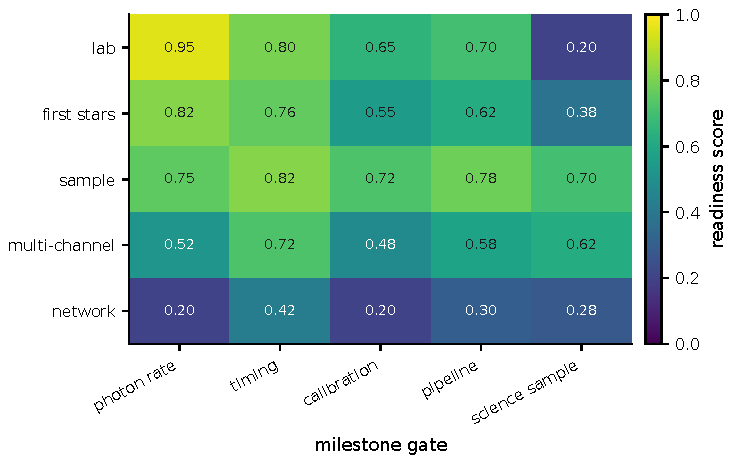
\includegraphics[width=0.90\linewidth]{figures/generated/chapter_22/ch22_milestone_gates.pdf}
\caption{不同阶段的里程碑门槛矩阵。课程实验与第一代恒星强度干涉在光子率、计时和 pipeline 上已较成熟，但多通道校准与网络阶段仍有明显缺口。图中的数字只是 proposal 里应当显式量化的 readiness score \emph{示例}，用来说明式 \eqref{eq:e28-milestone} 各项该怎样打分，并不代表任何设施承诺。}
\label{fig:e28-gates}
\end{figure}

再说风险。风险登记的精髓，是把风险和\textbf{失败判据}（failure criterion）绑在一起写：不仅说"可能出什么问题"，还要说"出到什么程度就该改方案、改到什么"。几个具体例子，都可以用前面的公式量化：若目标星比预期暗 1 mag，由式 \eqref{eq:e28-snr} 光子流下降、信噪比掉到约 \(40\%\)——缓解方案是预先备好更亮的替补目标或延长机时。若系统误差地板停在 \(\sigma_{\rm sys}\sim3\times10^{-5}\)，由式 \eqref{eq:e28-error-budget} 许多 \(|V|^2\) 小信号会被这一项淹没——缓解方案是先建校准星库把 \(\sigma_{\rm cal}\) 压下去。若一次 Type Ia 触发晚了 10 天，外壳更大但光度已下降、模型不确定性 \(\sigma_{\rm model}\) 上升——缓解方案是把触发响应写成硬指标、并对晚到事件设明确的放弃标准。若量子网络链路每天只给出很少的高保真纠缠对，就应把科学模式\textbf{退回}本地模式排序或常规强度干涉，而不是硬撑网络方案（第 \ref{chap:e24} 章）。

\begin{figure}[tbp]
\centering
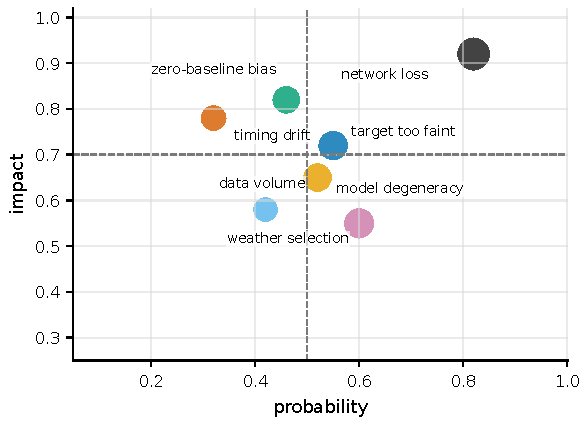
\includegraphics[width=0.86\linewidth]{figures/generated/chapter_22/ch22_risk_register.pdf}
\caption{路线图的风险登记图。横纵轴分别是发生概率与影响，点越大表示现有缓解方案越弱。右上角的风险必须在项目开始前配套缓解：网络损耗要先做短基线 pathfinder，零基线偏差要先建校准星库，目标过暗要预设明确的触发与放弃标准。}
\label{fig:e28-risk}
\end{figure}

这两件事合起来传达一个也许是本章最重要的态度：\textbf{好的研究计划允许自己失败，但要让每一次失败都告诉下一阶段该改什么}。检出为零的一夜，只要留下了定标好的事件表、通过的 null test 和一版公开相关器，就把仪器知识往前推了一步——这远胜于一个"只报告成功"的计划。

\section{把全书串成一条路径：从课程项目到研究课题}
\label{sec:e28-path}

最后，把前面六步拧成一根绳，看看它怎样从一个课堂练习，一路长成一份能提交的研究计划——以及在这条路上，量子网络这类远期设想该被摆在哪里。

起点可以很小。课程项目（第 \ref{chap:e26} 章）从桌面 HBT、事件表模拟、均匀圆盘拟合、SPADE 的 Fisher 信息（第 \ref{chap:e12} 章）和假警报计算开始——这些练习看似玩具，却已经把"提出问题 \(\to\) 设计观测 \(\to\) 估精度 \(\to\) 写计划"这条路径走了一遍缩微版。往上一层，较小的研究题目适合围绕\textbf{一个 pipeline}展开：时间同步、相关器、校准库、目标样本，或一个 open-data notebook——每一个都能独立成篇，也都留得下可复用的产出。再往上，较完整的科学题目可以瞄准 Be 星 \(\mathrm{H}\alpha\) 盘的谱线角尺度、快速自转星的多基线模型、Crab 脉冲星的相位分辨光子统计、Type Ia 距离 toy model 的系统误差，或本地模式排序（第 \ref{chap:e12} 章）与自适应光学的联合实验。最上层，大型合作再把这些课题接到 CTAO/IACT、ELT/VLTI/CHARA、Rubin、SKA、引力波网络，乃至量子网络实验室。

关于\textbf{远期}——量子网络望远镜何时才是主线——计划里要诚实地分层。很多信息学上的好处并不需要完整的量子网络：本地模式排序和相位敏感测量（第 \ref{chap:e12} 章）就能提高小分离、亮度矩估计的信息效率，这是\textbf{现在}就能推进的 \citep{2016PhRvX...6c1033T,2017PhRvL.118g0801T}。two-photon astrometry、单光子辅助或线性光学 pathfinder，目标是把天文光和实验室量子资源稳定地耦合起来，属于中期 \citep{2023PhRvL.130p0801M,2024SPIE13095E..1NR}。真正的纠缠辅助长基线干涉，则需要纠缠分发率、量子存储时间、频率转换效率、Bell 保真度和天文同步\textbf{同时}达标，属于更后面的阶段 \citep{2025PhRvA.111d3701M,2026PhRvA.113a2608P}。这套资源门槛在第 \ref{chap:e24} 章已经写成链路率、存储时间和有效保真度的约束；写计划时只需记住一个数量级：基线 \(B=1000\,\mathrm{km}\) 时光行时 \(B/c\simeq3.3\,\mathrm{ms}\)，地面 km 级基线只要 \(\mu\mathrm{s}\) 到 ms 级同步，但全球或空间基线会把存储与分发压力迅速放大。链路损耗、存储退相干、有用光子率任何一项不达标，网络方案就还不足以取代常规强度干涉——这时诚实的计划应当退回近期能做的那一档，而不是在 proposal 里透支未来。

\begin{figure}[tbp]
\centering
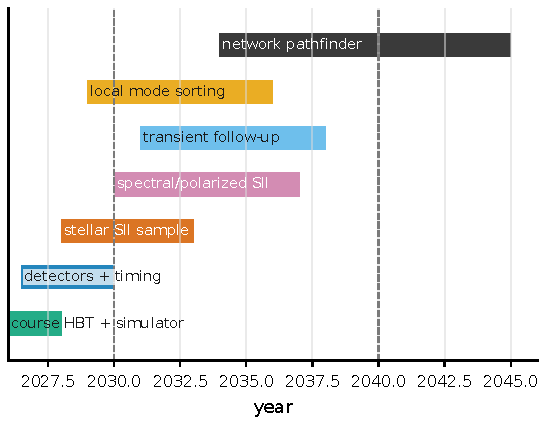
\includegraphics[width=0.92\linewidth]{figures/generated/chapter_22/ch22_program_timeline.pdf}
\caption{从课程 HBT 到量子网络 pathfinder 的阶段性时间线。早期任务建立人才、事件表、计时与校准；中期任务产出第一代科学样本与多通道相关；远期任务只有在本地模式排序、链路与存储指标达标后，才应写成设施级路线。这张时间线正是本章那条"从课程项目长成研究课题"的路径。}
\label{fig:e28-timeline}
\end{figure}

把这一切压成一句可操作的验收标准：\textbf{一份合格的研究计划，至少要列出新增的可观测量、事件表字段、数据估计步骤、每个符号的单位与典型范围、两个以上 null test，以及失败之后仍能留下的数据、代码或仪器约束}。满足这些，你的计划就能被复现、被审查、被改进；否则，"量子"二字就只停留在题目上，没有落到任何一个能被证伪的数字里。这，正是整本书想教给你的最后一件事：把工具变成问题，把问题变成观测，把观测变成一份别人能接着往下做的计划。

\section*{本章要点}
\addcontentsline{toc}{section}{本章要点}

\begin{itemize}
  \item \textbf{顺序不能反。} 先提科学问题、再定可观测量、最后才谈仪器与精度。选目标除了亮度、角尺度、外部先验，还要多问一条："失败后是否仍有产出？"
  \item \textbf{成熟度要可验收。} 用比值向量 \eqref{eq:e28-readiness} 给近期项目打分：光子率、计时、零基线对比度、系统误差、校准样本必须\textbf{同时}达标，任何一项 \(<1\) 都是必须先补的短板。
  \item \textbf{误差预算是地基。} 独立误差按方差相加（式 \eqref{eq:e28-error-budget}），最大项一票否决；统计噪声可用式 \eqref{eq:e28-snr} 估算，信噪比只随 \(\sqrt{\Delta f\,T}\) 增长，精度翻倍要四倍机时，这条要写进可行性小节（第 \ref{chap:e15} 章）。
  \item \textbf{数据流程要工程化。} 把数据产品写成集合 \eqref{eq:e28-data}：延迟直方图、\(|V|^2\)、跨通道协方差与完整协方差矩阵；定义好格式，教学、pathfinder 与主设施才能共用同一套事件表（第 \ref{chap:e13}、\ref{chap:e14} 章）。
  \item \textbf{里程碑与风险同写。} 里程碑五元组 \eqref{eq:e28-milestone} 同时钉住观测量、精度、时间、null test 数与交付；风险要连着失败判据一起写，让计划可以失败，但失败得告诉下一阶段该改什么。
  \item \textbf{远期要诚实分层。} 本地模式排序现在就能做，pathfinder 是中期，纠缠辅助网络要多项指标同时达标才是主线（第 \ref{chap:e24} 章）；不达标就诚实退回近期能做的那一档。
\end{itemize}

\medskip
\noindent\textbf{想一想}
\begin{itemize}
  \item 你手上有一个成熟度向量 \eqref{eq:e28-readiness}，其中光子率一项是 \(R_\gamma/R_{\rm req}=4\)，其余四项都在 \(0.9\) 左右。这个项目该不该现在就写成 proposal？如果不该，你会先把机时和经费投到哪一项上？
  \item 用式 \eqref{eq:e28-snr} 估一估：若把电子带宽 \(\Delta f\) 从 \(200\,\mathrm{MHz}\) 提到 \(800\,\mathrm{MHz}\)，在其余条件不变时，达到同样信噪比所需的积分时间大约缩短到原来的几分之几？
  \item 给你自己选一个第 \ref{chap:e25} 章里的科学案例，试着把它写成一个里程碑五元组 \eqref{eq:e28-milestone}：它的 \(O_j\)、\(\sigma_{O,j}^{\rm goal}\)、\(N_{{\rm null},j}\) 和 \(D_{{\rm release},j}\) 分别该填什么？哪一项你现在还答不上来，说明计划还缺哪一步？
\end{itemize}
